\section{Introduction}
\label{sec:introduction}

In recent years, quantum computing has transitioned from a theoretical concept~\cite{feynman2018simulating} to a rapidly maturing technology that garners academic research~\cite{gracejohnson2022} and industrial interest. According to the MIT Quantum Index Report 2025 \cite{ruane2025quantum}, the field is experiencing an unprecedented expansion in hardware availability, corporate communications, and global intellectual property, evidenced by a fivefold increase in quantum technology patents over the past decade. The rapid development of commercial Quantum Processing Units (QPUs) highlights the urgent need for hybrid infrastructure capable of orchestrating classical and quantum workloads.

\begin{figure*}[h]
    \centering
    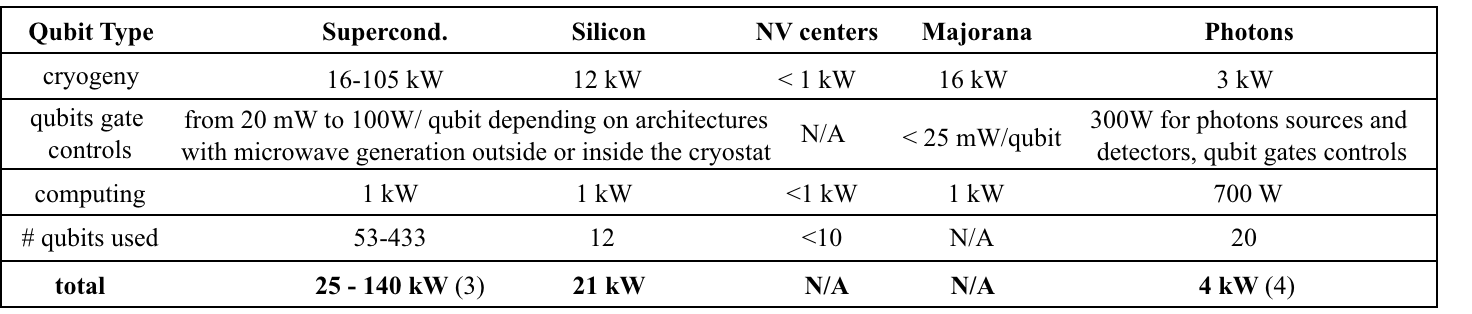
\includegraphics[width=\textwidth]{Images/energy_usage-compact.png}
    \caption{Energetic requirements and architectural comparison of quantum computing modalities (source: Ezratty et al.~\cite{ezratty2021}).}
    % \Description{}
    \label{fig:energy_usage}
\end{figure*}

However, raw quantum advantage cannot be realized in isolation. Modern quantum algorithms, such as the Variational Quantum Eigensolver (VQE)~\cite{peruzzo2014vqe}, Quantum Approximate Optimization Algorithm (QAOA), and Quantum Neural Networks (QNNs), are inherently hybrid. These workloads depend on tight feedback loops where classical High Performance Computing (HPC) nodes handle statevector simulation, parameterized circuit compilation, and numerical optimization, while the QPUs execute quantum state preparations and measurements. As a result, the ultimate system throughput is constrained not only by QPU fidelity or qubit counts, but also by the efficient orchestration, dynamic scheduling, and data transfer overheads between classical CPU resources and heterogeneous QPU coprocessors.

This work is motivated by the need to model and quantify energy and power consumption within hybrid quantum cloud architectures. Because physical hardware access is constrained and energy dynamics in hybrid environments are complex, simulation serves as a vital tool. It allows researchers and system architects to model complex execution workflows, test scheduling hypotheses, and predict performance and energy metrics across scale. To bridge this critical tooling gap, this paper leverages HybridCloudSim, a discrete event simulation framework engineered to model, evaluate, and optimize hybrid classical quantum cloud environments. HybridCloudSim connects algorithmic specifications and physical hardware dynamics by establishing capacity aware models for both CPU clusters and QPU hardware pools. 

Our contributions in this paper are as follows:

\textbf{Unified resource scheduling and brokerage.} A broker that schedules concurrent, heterogeneous jobs under strict capacity constraints, allocating CPU cores and memory bandwidth classically while resolving quantum allocation at two levels, namely aggregate qubit capacity and physical connectivity, so that fragmentation effects invisible to qubit count only models are exposed.

\textbf{Energy and power accounting.} A configurable cost model that attributes energy per execution phase from device specific power profiles drawn from Ezratty et al.~\cite{ezratty2021} as the ground truth.

\textbf{Integrated telemetry and monitoring.} An event driven monitor that records device utilization, instantaneous fleet power, and queueing behavior at event boundaries, producing traces that support analysis over the run itself rather than end of run aggregates.

Through a series of simulation studies, we demonstrate how HybridCloudSim enables system architects to locate hardware bottlenecks, compare dynamic scheduling policies, and reason about the energy and cost implications of resource allocation in emerging hybrid cloud infrastructures. In particular, we show that energy and power aware simulation provides a principled basis on which researchers and cloud operators can set pricing policy, by varying device configurations and workload parameters within the framework rather than by procuring physical hardware. This work demonstrates that simulation models can assist researchers and cloud administrators in establishing pricing based on energy and power consumption by adjusting parameters and configurations directly within the framework. Detailed circuit execution is deliberately abstracted away, allowing the framework to act as a lightweight digital twin of a hybrid quantum classical cloud. As this work targets orchestration level modeling, we refer the reader to Nielsen and Chuang~\cite{nielsen2010quantum} for a detailed introduction to quantum computation and quantum information theory.
